\documentclass[a4paper,12pt,titlepage,openany]{book}
\usepackage[utf8]{inputenc}
\usepackage[italian]{babel}
\usepackage[noadvisor]{frontespizio}
\usepackage{amsmath}
\usepackage{amsthm}
\usepackage{amssymb}
\usepackage{mathptmx}  % Font
\usepackage{dashbox}   % Dashed box for math equations
\usepackage[linktocpage=true,hyperfootnotes=false,colorlinks=true,linkcolor=orange]{hyperref}  % Link nell'indice
\usepackage{microtype} % migliora l'uso di spazi e rientri
\usepackage{bbding}    % New symbols for itemize
\usepackage{setspace}  % Permette di personalizzare l'interlinea
\usepackage{fancyhdr}  % Gestione headings
\usepackage{graphicx}  % Permette di includere figure
\usepackage{booktabs}  % Creazione tabelle
\usepackage{caption}   % Permette la personalizzazione delle didascalie e la loro aggiunta in tabelle
\usepackage[wide]{sidecap}  % Permette di mettere didascalie laterali a figure e tabelle
\usepackage{subfig}    % Crea sottofigure o sottotabelle
\usepackage[]{xcolor}  % Add colors

% Theorems setup
\newtheoremstyle{mydef}
{\topsep}{\topsep}%
{\leftskip=2em\rightskip=2em}{}%
{\scshape}{}%
{\newline}%
{\textbf{\thmname{#1}~\thmnumber{#2}}\thmnote{\ -\ #3}.}

\theoremstyle{mydef}
\newtheorem{definizione}{Definizione}[chapter]

% Pagestyle
\pagestyle{fancy}
\renewcommand{\headrulewidth}{0pt} % no rule at the top
\fancyhf{} % clear all fields
\fancyhead[LO,RE]{\small\bfseries\nouppercase{\leftmark}}
\fancyhead[RO,LE]{\small\bfseries\thepage}

% Other little adjustments
\renewcommand\thefootnote{\textcolor{black}{\arabic{footnote}}}
\renewcommand\labelitemi{\footnotesize\NibSolidRight}
\newcommand\dboxed[1]{\dbox{\ensuremath{#1}}}  % Allow dbox to be used in math env
\linespread{1.2}
\captionsetup{format=hang, labelfont={sf,bf}}
\sidecaptionvpos{figure}{c}  % Side caption centered to image

\begin{document}
	\begin{frontespizio}
        \Preambolo{\usepackage{romannum}}
		\Universita{Verona}
        \Dipartimento{Informatica}
		\Corso[Laurea Triennale]{Informatica}
		\Annoaccademico{2017--2018}
		\Titoletto{Progetto di \LaTeX}
		\Titolo{Appunti di fisica II}
		\Sottotitolo{Riassunto del corso di elettromagnetismo\\ 
                     e raccolta di formule utili per l'esame}
		\NCandidato{Studente}
        \Candidato[VR398611]{Michele Martini}
	\end{frontespizio}
    
    \frontmatter
    \pagestyle{plain}
    \cleardoublepage
    \tableofcontents
    \listoffigures
    \listoftables
    \cleardoublepage

    \chapter*{Introduzione} \addcontentsline{toc}{chapter}{Introduzione}
    \chaptermark{INTRODUZIONE}
        Il presente scritto non vuol essere una formale dispensa per il corso di fisica II,
        bensì una semplice raccolta di appunti presi a lezione, sistemati e migliorati nella
        forma e nel contenuto.
        
        Verranno dunque presentati gli argomenti nello stesso ordine con il quale sono stati
        affrontati durante le ore in università, introducendo come prime grandezze fisiche la carica
        elettrica ed il potenziale, che forniranno una solida base per poter argomentare adeguatamente
        l'elettrostatica nel vuoto.\\
        Proseguiremo successivamente trattando l'elettrodinamica, il magnetismo ed infine, unendo le
        nozioni apprese da ambo le parti, si chiuderà il cerchio trattando quindi l'elettromagnetismo.\\
        \emph{Nota:} gli argomenti verranno studiati quasi unicamente in forma integrale, approfondendo solo
        in taluni momenti la natura locale dei fenomeni analizzati.
        
        \bigskip
        La maggior parte dei fenomeni che studieremo verrà introdotta da cenni storici ed, eventualmente,
        dall'esperimento che ne ha segnato l'effettiva scoperta. Questo metodo può rivelarsi utile per vari motivi,
        tra i quali:
        \begin{enumerate}
            \item memorizzare più facilmente i passi scientifici fondamentali su cui si basa l'odierno elettromagnetismo;
            \item osservare come e con quale scopo si progettano veri e propri esperimenti di fisica;
            \item scoprire qualche nuovo, interessante aneddoto per fare colpo sulle ragazze.
        \end{enumerate}
        
        \bigskip
        \begin{center}
            Nella speranza che questo piccolo fascicolo possa esservi di qualche utilità,
            vi~auguro~\emph{buona~lettura!}
        \end{center}


    \mainmatter
    \pagestyle{fancy}
    \chapter{Elettrostatica nel vuoto}
        Nel corso dei secoli, grazie all'impegno ed agli importanti studi di innumerevoli personaggi,
        siamo giunti a racchiudere le nostre attuali conoscenze fisiche dell'universo in un unico
        modello, denominato \emph{``modello standard''}. Secondo la teoria da esso descritta,
        esistono 4 interazioni
        fondamentali, ovvero:
        \begin{itemize}
            \item forza di gravità;
            \item forza elettromagnetica;
            \item forza nucleare forte;
            \item forza nucleare debole.
        \end{itemize}
        Il MS ci dice inoltre che ognuna di esse agisce tramite un \emph{campo}; in questo capitolo studieremo
        il \emph{campo elettrico}. Tuttavia, per motivi che saranno più chiari solo nei capitoli successivi del libretto, lo studieremo in una situazione particolare, ovvero in condizioni \emph{stazionarie} (o \emph{statiche}).
        \footnote{Fenomeni non influenzati dal tempo}
        
        \section{La carica elettrica}
            Con svariati esperimenti, taluni anche molto semplici, si può facilmente osservare che ogni materiale
            può essere elettrizzato tramite strofinio, contatto o induzione elettrica. Ciò permise di supporre
            l'esistenza di una proprietà intrinseca della materia. Quest'ultima è la \emph{carica elettrica},
            e si misura in \emph{Coulomb} $[C]$.\footnote{Grandezza derivata: $1A=1C/1s$}
            
            Un'importante caratteristica della carica consiste nel fatto che sia quantizzata, infatti ha sempre valore
            multiplo di $e$.\footnote{Carica di un elettrone ($1,6022 \times 10^{-19}C$)}
            La carica di un materiale può essere inoltre positiva o negativa, e possiamo osservare quanto segue:
            \begin{itemize}
                \item cariche con segno concorde si respingono;
                \item cariche con segno discorde si attraggono.
            \end{itemize}
            \begin{figure}[htp]
                \centering
                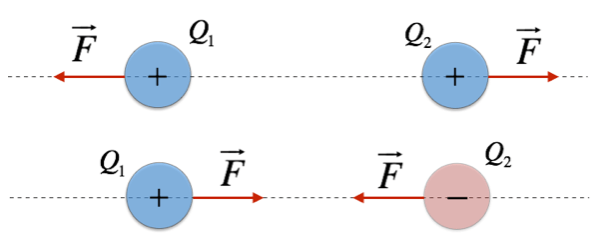
\includegraphics[width=0.5\textwidth]{forza_coulomb}
                \captionsetup{width=0.6\textwidth, justification=raggedright}
                \caption[Attrazione/repulsione tra due cariche]{Cariche discordi di attraggono, cariche concordi si respingono.}
            \end{figure}
            Alla luce di ciò, possiamo finalmente pensare ad esperimenti pratici (con ``proprietà intrinseche'' si
            ragiona poco, ma con le forze è tutta un'altra storia!).
        
        \section{Forza di Coulomb e campo elettrostatico}
            La forza repulsiva/attrattiva che si verifica tra corpi ``carichi'' (analizzeremo in dettaglio tale
            termine in seguito) ha particolari caratteristiche, che furono studiate in modo appofondito da Charles
            Augustin de Coulomb (1736-1806) nel suo famoso esperimento eseguito con la bilancia di torsione.\\
            Sappiamo che:
            \begin{itemize}
                \item $F \propto q_1q_2$
                \item $F \propto \frac{1}{r^2}$
                \item $F$ centrale
            \end{itemize}
            Partendo da tali osservazioni, possiamo definire la forza di Coulomb.
            \begin{definizione}[Legge di Coulomb]
                Due cariche si attraggono o si respingono con una forza che agisce lungo la congiungente i centri
                dei due corpi, con intensità direttamente proporzionale alle cariche e inversamente proporzionale
                al quadrato della loro distanza.
                \begin{align}
                    \vec{F}_{1,2}=K\frac{q_1q_2}{r_{1,2}^2} \vec{u}_{1,2}\text{,}\quad
                    \text{con } k=\frac{1}{4\pi\epsilon_0}
                \end{align}
            \end{definizione}
            \noindent
            Nella definizione della forza di Coulomb incontriamo inoltre, per la prima volta, la costante $\epsilon_0$,
            \footnote{$\epsilon_0$: permittività elettrica del vuoto ($8,8541\times 10^{-12}F/m$).} la quale ci 
            accompagnerà in quasi ogni formula che analizzeremo.
            
            \emph{Vale il principio di sovrapposizione}: la forza agente tra due cariche non viene influenzata da
            eventuali altre forze presenti nel sistema ed agenti sulle medesime cariche. Con questa premessa risulta
            più che umano analizzare un sistema di $N$ cariche puntiformi.
            \begin{align*}
                \vec{F}_{tot_{q_0}} = \sum_{1}^{N}{\vec{F}_{i_0}} =
                &\underbrace{\frac{1}{4\pi\epsilon_0}\sum_{1}^{N}{\frac{q_iq_0}{r_{i,0}^2}\vec{u}_{i,0}}} =
                \frac{q_1q_0}{4\pi\epsilon_0r_{1,0}^2}\vec{u}_{1,0} + \dotsb\\
                &\vec{F}_{tot_{q_0}} = 
                \frac{\mathbf{q_0}}{4\pi\epsilon_0}\sum_{1}^{N}{\frac{q_i}{r_{i,0}^2}\vec{u}_{i,0}}\\
                &\vec{F}_{tot_{q_0}} = 
                q_0\cdot\frac{1}{4\pi\epsilon_0}\sum_{1}^{N}{\frac{q_i}{r_{i,0}^2}\vec{u}_{i,0}} =
                q_0\cdot\vec{E}(\vec{r})
            \end{align*}
            \begin{definizione}[Campo elettrostatico]
                Il campo elettrostatico $\vec{E}(\vec{r})$ è definito come la forza per unità
                di carica alla quale è soggetta una carica puntiforme $q_0$ se posta in posizione $\vec{r}$.
                \begin{align}
                    \boxed{\vec{E}(\vec{r}) = \frac{\vec{F}}{q_0}}
                \end{align}
                Tale campo è dunque una \emph{proprietà dello spazio}.
                La sua unità di misura è $[V/m]$ (oppure, ricavandola dalla formula: $[N/C]$).
            \end{definizione}
            
            \noindent
            Le linee di campo escono dalle cariche positive, dette \emph{``sorgenti''}, ed entrano nelle cariche
            negative, dette \emph{``pozzi''}.
            Sia linee di campo di $\vec{E}(\vec{r})$ sia le linee di forza della $\vec{F}$
            di Coulomb sono radiali, con centro nella sorgente del campo, e dunque parallele tra loro.
            \begin{figure}[htp]
                \centering
                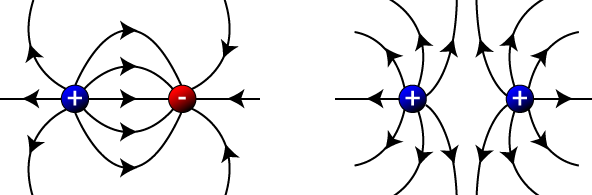
\includegraphics[width=0.7\textwidth]{linee_campo}
                \caption{Linee di campo di $\vec{E}$.}
            \end{figure}
            
            \subsection{Energia e potenziale elettrostatico}
            La forza elettrostatica è \emph{conservativa}, quindi: $\exists\,U\mid W=-\Delta U$.\\
            Posta una carica positiva $Q$ nell'origine e una carica $q_0$ in un punto A, il lavoro per spostare
            $q_0$ da A ad un punto B e l'energia elettrostatica delle due cariche si calcolano come segue:
            \begin{gather}
            \vec{F}_{el.st.}(r) = q_0\frac{Q}{4\pi\epsilon_0r^2}\vec{u}_r \notag \\[1ex]
            \begin{aligned}
            W_{AB} &= \int_{AB}\vec{F}_{el.st.}\cdot\,d\vec{s}
            = \int_{AB}\frac{q_0Q}{4\pi\epsilon_0r^2}\,\vec{u}_r\,d\vec{s}
            = \int_{r_A}^{r_B}\frac{q_0Q}{4\pi\epsilon_0r^2}\,dr \\
            &= -\frac{q_0Q}{4\pi\epsilon_0r}\biggr\rvert_{r_A}^{r_B}
            = -\frac{q_0Q}{4\pi\epsilon_0r_B} + \frac{q_0Q}{4\pi\epsilon_0r_A} = -\Delta U
            \end{aligned}
            \notag\\[1ex]
            \dboxed{U = \frac{q_0q_1}{4\pi\epsilon_0r} + \text{cost}}
            \end{gather}
            \begin{definizione}[Potenziale del campo elettrostatico]
                Il potenziale elettrostatico si definisce come l'energia potenziale elettrostatica per unita di carica.
                La sua unità di misura è il \emph{Volt} $[V]$ ed il suo valore è definito a meno di una costante.
                \begin{equation}
                    \boxed{V\triangleq U/q}\\
                \end{equation}
            \end{definizione}
    
    \chapter{Elettrodinamica}
        In questo capitolo studieremo i fenomeni elettrici in condizioni \emph{non stazionarie}, introducendo la \emph{corrente elettrica} e studiandone il comportamento nei conduttori.
        
        \section{Conduzione elettrica}
            All'interno dei metalli, gli elettroni di valenza sono liberi di muoversi e non sono legati ad un atomo
            specifico. Energia cinetica media di tali cariche è data dall'\emph{``agitazione termica''}:
            \begin{align}
                \overline{E}_K &= 3K\frac{T}{2} \notag \\
                &= \frac{1}{2}\,m\,\overline{v}^2 \label{eqn:vel_termica}
            \end{align}
            La $v$ presente in \ref{eqn:vel_termica} è la \emph{velocità termica} delle particelle: ha direzione casuale
            e misura circa $1,2\times 10^5 m/s$.\footnote{In un conduttore con temperatura $300K$.}
            
            Se immergiamo il metallo in un campo $\vec{E}$ generiamo un moto ordinato nella nuvola di elettroni,
            detto \emph{velocità di deriva}: essa ha una direzione ben precisa ed una velocità generalmente molto
            più bassa rispetto a quella termica (una differenza di svariati ordini di grandezza!).\\
            Tale moto ordinato è chiamato \emph{``conduzione elettrica''} o \emph{``corrente''}.
            
            \begin{definizione}[Corrente]
                Moto ordinato degli elettroni di un conduttore. Considerando un conduttore di sezione $S$ percorso da
                corrente, l'intensità di quest'ultima si misura in \emph{Ampere} $[A]$ e si definisce come la quantità
                di carica $dQ$ che attraversa la superficie $S$ in un intervallo di tempo $dt$:
                \begin{equation}
                    \boxed{I = \frac{dQ}{dt}}
                \end{equation}
                Per convenzione e ragioni storiche si indica con segno positivo il verso di moto delle cariche positive.
            \end{definizione}
            
            \begin{SCfigure}[0.3][htp]
                \centering
                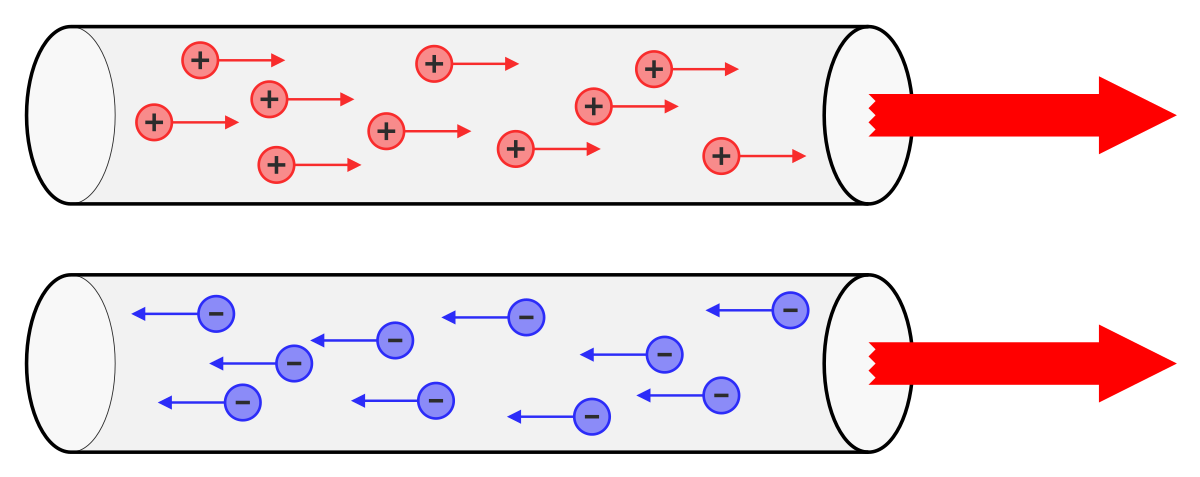
\includegraphics[width=0.7\textwidth]{corrente_elettrica}
                \captionsetup{format=plain, justification=raggedright,labelsep=newline}
                \caption{Segno della corrente elettrica\\ secondo la convenzione.}
            \end{SCfigure}
            
            \noindent
            Conoscendo l'intensità di corrente $I$ che scorre in un conduttore, data una superficie $S$, possiamo ricavarne
            la \emph{densità di corrente $\vec{J}$}.
            \begin{align}
                I = \int_{\sup}\vec{J}\cdot\,d\vec{S}& \notag\\
                \text{Flusso attraverso} & \text{ la superficie} \notag\\
                \overbrace{\,n\cdot e\cdot\vec{v}\cdot d\vec{S}\,} = &\frac{dq}{dt} \text{\ ,\ \ dove }
                n =\frac{\text{\# elettroni}}{\text{volume}} \notag\\[1em]
                \dboxed{\vec{J} = n\cdot e\cdot\vec{v}} & \qquad \dboxed{J = \frac{I}{\Sigma}}
            \end{align}

    \chapter{Magnetostatica}
        Evidenze osservate nei vari esperimenti:
        \begin{itemize}
            \item alcuni materiali (composti da magnetite) possono attirare altri materiali (ferrosi);
            \item alcuni materiali si orientano lungo una direzione privilegiata;
            \item i fenomeni attrattivi/repulsivi di cui sopra si manifestano sui bordi ($\vec{F}$~localizzata);
            \item \emph{non esistono cariche magnetiche isolate}. Coulomb tentò di riprodurre lo stesso esperimento
                della bilancia di torsione, ma senza alcun risultato;
            \item se spezzo un magnete, ottengo due nuovi magneti: esistono solo dipoli magnetici;
            \item \emph{esperimento di \O{}rsted} permise di scoprire che le correnti sono sorgenti del campo magnetico;
            \item ad Ampere dobbiamo la scoperta che queste sono le \emph{uniche} sorgenti del campo magnetico.
        \end{itemize}
    
    \appendix
    \chapter{Costanti fisiche}
        \begin{table}[h]
            \caption{Principali costanti fisiche.}
            \centering
            \begin{tabular}{lcrc}
                \toprule
                Costante fisica & Simbolo & Valore & Unità di misura\\
                \midrule
                Velocità della luce nel vuoto & $c$ & $299\,792\,458$ & $m\,s^{-1}$\\
                Costante di Plank & $h$ & $6,6260\times 10^{-34}$ & $J\,s$\\
                Carica dell'elettrone & $e$ & $1,6022\times 10^{-19}$ & $C$\\
                Massa dell'elettrone & $m_e$ & $9,1094\times 10^{-31}$ & $kg$\\
                Costante dielettrica del vuoto & $\epsilon_0$ & $8,8542\times 10^{-12}$ & $F\,m^{-1}$\\
                Permeabilità magnetica del vuoto & $\mu_0$ & $12,5664\times 10^{-7}$ & $N\,A^{-2}$\\
                Costante di Boltzman & $k$ & $1,3807\times 10^{-23}$ & $J\,K^{-1}$\\
                Numero di Avogadro & $N_A$ & $6,0221\times 10^{-23}$ & mol$^{-1}$\\
                \bottomrule
            \end{tabular}
        \end{table}
    
    \chapter{Costanti dielettriche e magnetiche}
        \begin{table}[ht]
            \captionsetup{width=0.7\textwidth}
            \caption{Costante dielettrica relativa e permeabilità magnetica relativa di alcune sostanze.}
            \centering
            \subfloat[][\emph{Costanti dielettriche relative di alcune sostanze.}]{
                \begin{tabular}{lc}
                    \toprule
                    Materiale & Costante dielettrica relativa $[\epsilon]$\\
                    \midrule
                    Vuoto & $1$\\
                    Aria secca & $1,00059$\\
                    Elio & $1,00087$\\
                    Acqua & $80$\\
                    Glicerina & $43$\\
                    Benzene & $3,1$\\
                    Carta & $3,5$\\
                    Polistirolo & $2,6$\\
                    Bachelite & $4,9$\\
                    \bottomrule
                \end{tabular}
            }
            \subfloat[][\emph{Permeabilità magnetica relativa di alcune sostanze.}]{
                \begin{tabular}{lc}
                    \toprule
                    Materiale & Permeabilità magnetica relativa $[\mu]$\\
                    \midrule
                    Vuoto & $1$\\
                    Oro & $0,999964$\\
                    Argento & $0,999974$\\
                    Rame & $0,9999902$\\
                    Acqua & $0,9999912$\\
                    Aria & $1,0000004$\\
                    Platino & $1,000360$\\
                    Ferro & $5,50$\\
                    Permalloy & $25,00$\\
                    \bottomrule
                \end{tabular}
            }
        \end{table}
\end{document}




